\begin{problem}{}{input.png}{}{2 секунди}{256 мегабайт}
% OpenCV: Counting problem}

Важливість розпізнавання та підрахунку об'єктів стає дедалі важливішою у сучасному світі, 
де обробка зображень та комп'ютерний зір є ключовими аспектами технологічного розвитку.

В цій задачі треба обробляти зображення у форматі PNG.
Зображення містять прямокутники різних розмірів та кольорів, вони можуть бути обернені на довільний кут, мати заокруглені кути.
Гарантується, що прямокутники не перетинаються та не накладаються один на одного. 

Розробіть та реалізуйте алгоритм обробки заданого зображення для визначити кількості прямокутників на ньому.

\InputFile
Вашій програмі на вхід подається зображення \t{input.png}. 

\OutputFile
Виведіть одне ціле число $-$ кількість прямокутників на зображенні.

\Constraints
Нехай $W \times H$ $-$ розмір зображення, $a_i \times b_i$ $-$ розміри прямокутників.

$100 \le W \le 1\,000$

$100 \le H \le 1\,000$

$5 \le a_i \le 300$

$5 \le b_i \le 300$


\Examples
\begin{example}
\exmp{
\medskip
\begin{center}
  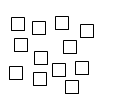
\includegraphics[width=0.60\textwidth]{exmp1.png}
\end{center}
}{12
}%
\exmp{
\medskip
\begin{center}
  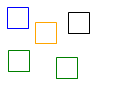
\includegraphics[width=0.60\textwidth]{exmp11.png}
\end{center}
}{5
}%
\exmp{
\medskip
\begin{center}
  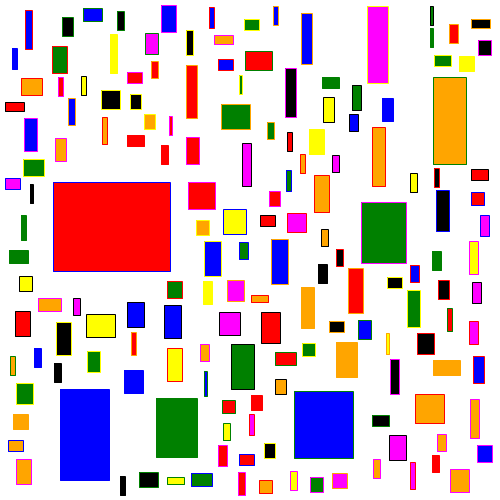
\includegraphics[width=0.60\textwidth]{exmp20.png}
\end{center}
}{165
}%
\exmp{
\medskip
\begin{center}
  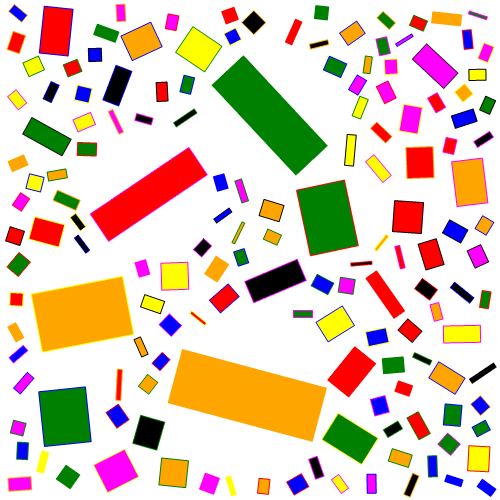
\includegraphics[width=0.60\textwidth]{exmp40.png}
\end{center}
}{154
}%
\exmp{
\medskip
\begin{center}
  
\includegraphics[width=0.60\textwidth]{exmp43.png}
\end{center}
}{37
}%
\end{example}

\end{problem}

